\chapter{Adaptive Mesh Refinement} \label{chapter:adaptive_mesh_refinement} 
% Something about move semantics
% No coarsening
% Adaptivity triggers
% Mortar here

Computers constantly increase in power, thanks to incremental progress made on known processes and
new architectures such as that described in Chapter~\ref{chapter:graphics_processing_units}.
However, processing power and memory is still limited and the size of problems studied has
increased in step with the available resources. It is still necessary to carefully manage those
limited resources in order to maximise the efficiency of simulations. Some flow regions may be more
interesting or harder to compute, benefiting from an increase in resolution. On the other hand, some
flow regions may have less happening in them or be easier to compute, and a decrease in resolution
may be acceptable.

\begin{figure}[H]
	\centering
	\subfloat[Mesh before refining]
	{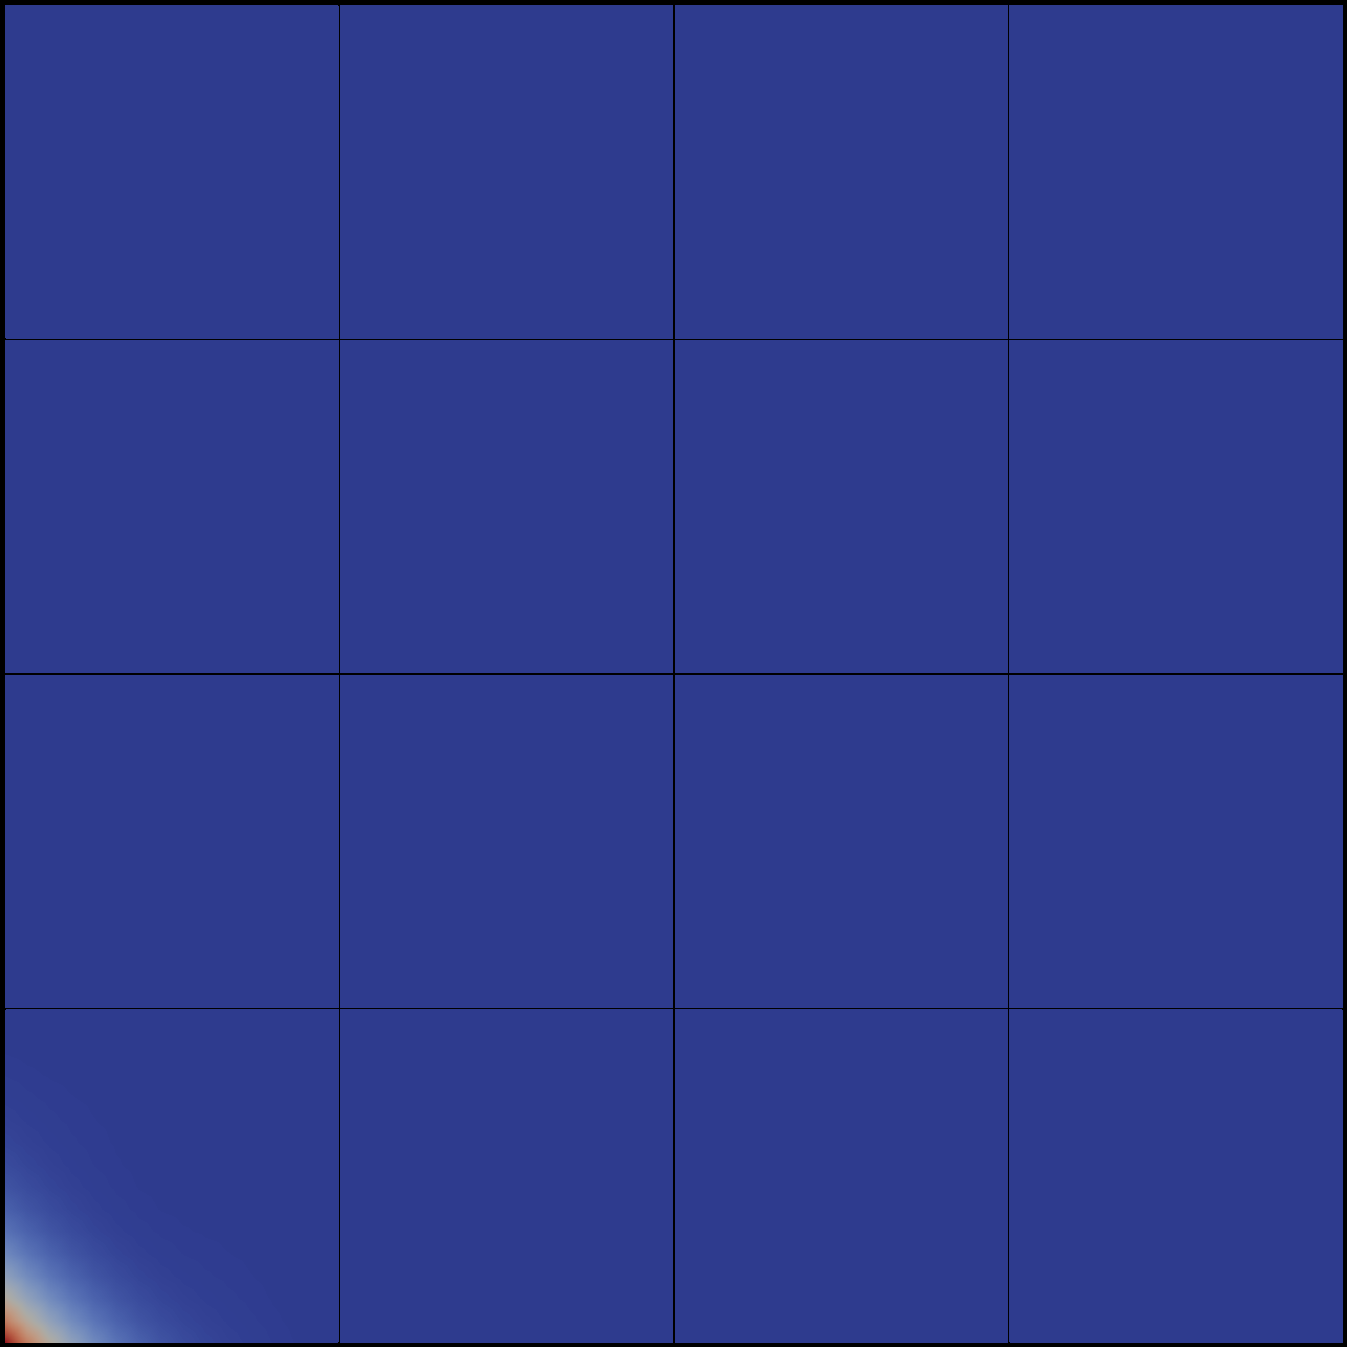
\includegraphics[width=0.45\textwidth]{Chapter_adaptive_mesh_refinement/media/mesh_initial} \label{fig:mesh_initial}}
	\hfill
	\subfloat[Mesh after refining]
	{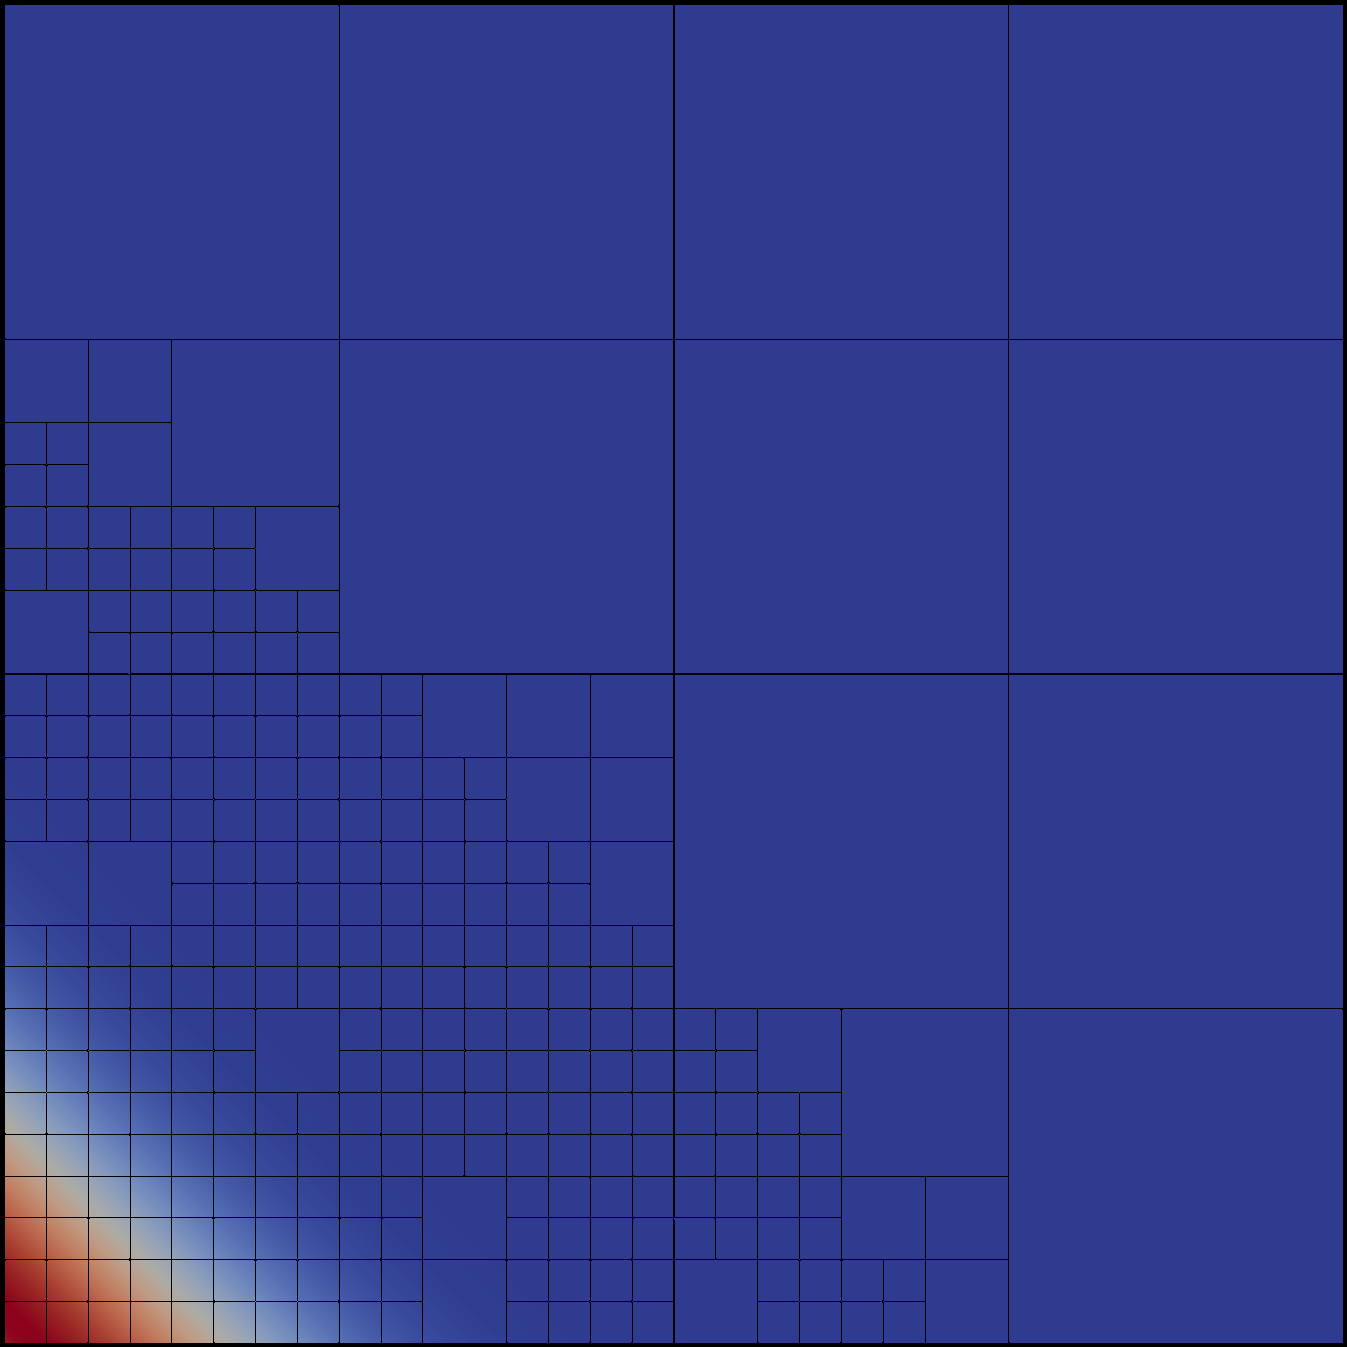
\includegraphics[width=0.45\textwidth]{Chapter_adaptive_mesh_refinement/media/mesh_refinement} \label{fig:mesh_after_refinement}}
	\caption{Adaptive mesh refinement: The elements have split near the wave, where the solution is steeper. (a) Before refining (b) After refining}.
	\label{fig:mesh_refinement}
\end{figure}

It is possible to increase the number of elements and/or the polynomial order of an entire mesh
before solving the problem. This increases resolution in important areas of the flow, but also
increases resolution everywhere else in the domain, where the increased computation cost provides no
benefit. It is sometimes possible to predict where to refine before solving the problem, such as
around static shock waves in predictable locations. In these cases, the mesh can be refined in those
areas before computation has started. However, it is not always possible to know these areas
beforehand, or these areas may move as time advances if the problem is transient. The error may also
be higher in unforeseen areas that are not apparent.

Adaptive mesh refinement is the process of mesh resolution as the computation goes, where the effect
of that increase in resolution is most needed. To find out where to refine, the solution error must
be estimated, and a refinement method must be chosen. The error can be estimated by extrapolating
the value of the next mode, and the slope of the last few modes can guide the choice of the
refinement method. The two refinement methods studied here are h-refinement and p-refinement,
increasing the number of elements and the polynomial order, respectively. 

This whole process must be executed in parallel and with as much as the work as possible executed on
the GPU. GPUs are more efficient at working with fixed workloads where all threads of a block
execute the same instruction. Refining the mesh moves memory around and can introduce additional
branching if the elements have different polynomial orders or non-conforming interfaces. The
adaptivity process itself is also hard to implement on GPUs, as elements must either move, change
their polynomial order or split into multiple elements in parallel. If the different threads are not
perfectly coordinated, they could do these operations on the same destination memory location,
creating race conditions.

Once the mesh has been refined, the element boundaries can become geometrically or functionally
non-conforming. To compute fluxes between the elements, we use the mortar element method. Mortar, in
the form of faces, is added between the elements, and the boundary solution is projected from the
elements to the face's own collocation points. 

When solving problems in parallel, the mesh will be split into blocks, each assigned to a process
and its GPU. As the mesh is refined, it is possible that the blocks are refined unequally. This can
lead to a load imbalance between the different GPUs. As the different GPUs need to synchronise at
each timestep, lightly-loaded GPUs will always be waiting after heavily-loaded GPUs. The computation
time will therefore be driven by the most heavily-loaded GPU, and the speedup incurred by
parallelizing the program will be reduced. To improve this side effect of mesh refinement, a dynamic
load balancing algorithm will be implemented in Chapter~\ref{chapter:load_balancing}.

\section{Strategies} \label{section:adaptive_mesh_refinement:adaptivity_strategies}

\subsection{p-adaptivity} \label{section:adaptive_mesh_refinement:adaptivity_strategies:p-adaptivity}

\begin{figure}[H]
	\centering
	\includesvg[width=0.6\textwidth]{Chapter_adaptive_mesh_refinement/media/p-adaptivity_N4_N6}
	\caption{2D p-adaptivity: The element's polynomial order is increased from 4 to 6, with 5 to 7 collocation points}
	\label{fig:p-adaptivity}
\end{figure}

The first refinement strategy is p-adaptivity. When refining this way, elements increase their
polynomial order to increase their resolution. The lower-order solution is projected to the
higher-order collocation points. In this work, the polynomial order in increased in steps of 2, and
is required to be identical in the x and y directions. 

\subsection{h-adaptivity} \label{section:adaptive_mesh_refinement:adaptivity_strategies:h-adaptivity}

\begin{figure}[H]
	\centering
	\includesvg[width=0.6\textwidth]{Chapter_adaptive_mesh_refinement/media/h-adaptivity_N4}
	\caption{2D h-adaptivity: The element splits into 4 elements}
	\label{fig:h-adaptivity}
\end{figure}

The second refinement strategy is h-adaptivity. h-adaptivity splits single elements into several
elements occupying the same space. In this work we exclusively deal with quadrilaterals, and these
elements split in 4 smaller elements when h-refining. The solution is projected from the initial big
element to each of the 4 offspring elements.

\subsection{hp-adaptivity} \label{section:adaptive_mesh_refinement:adaptivity_strategies:hp-adaptivity}

In order to maximise computation efficiency, both p-adaptivity and h-adaptivity are used together.
An hp-adaptive program uses either p-adaptivity or h-adaptivity on an element-by-element basis,
depending on which is expected to reduce error the most. The choice between the two methods is
detailed in Section~\ref{section:adaptive_mesh_refinement:refinement_criteria}.

\begin{figure}[H]
	\centering
	\includesvg[width=0.6\textwidth]{Chapter_adaptive_mesh_refinement/media/hp-adaptivity_N4_N6}
	\caption{2D hp-adaptivity: Elements refining create non-conforming interfaces}
	\label{fig:hp-adaptivity}
\end{figure}

Once the mesh has been refined, it is possible that the interfaces between elements become
non-conforming. Each interface is made up of two element edges, in bold black, and a face, in blue.
Recall from Chapter~\ref{chapter:spectral_element_method} that fluxes are computed between the
elements from the extrapolated values of the solution on collocation points corresponding to the
polynomial order of the elements. These would be sitting on the bold black lines in the figure
above. This works directly if two neighbouring elements have the same polynomial order and they
completely share an edge. However, after p-adaptivity, interfaces can become functionally
non-conforming, as seen with the horizontal blue line in the figure above. The nodes won't match
anymore since one element has more points than the other. After h-adapting, interfaces can become
geometrically non-conforming, as seen with the topmost blue line in the figure above. The nodes do
not match because one element edge is shorter than the other. Finally, interfaces can be both
geometrically and functionally non-conforming, as seen with the bottom blue line in the figure
above. We will have to find a way to connect those elements in a way that retains the spectral
convergence of the method. Such a method is described in
Section~\ref{section:adaptive_mesh_refinement:mortar_element_method}.

\begin{figure}[H]
	\centering
	\subfloat[Mesh before refining]
	{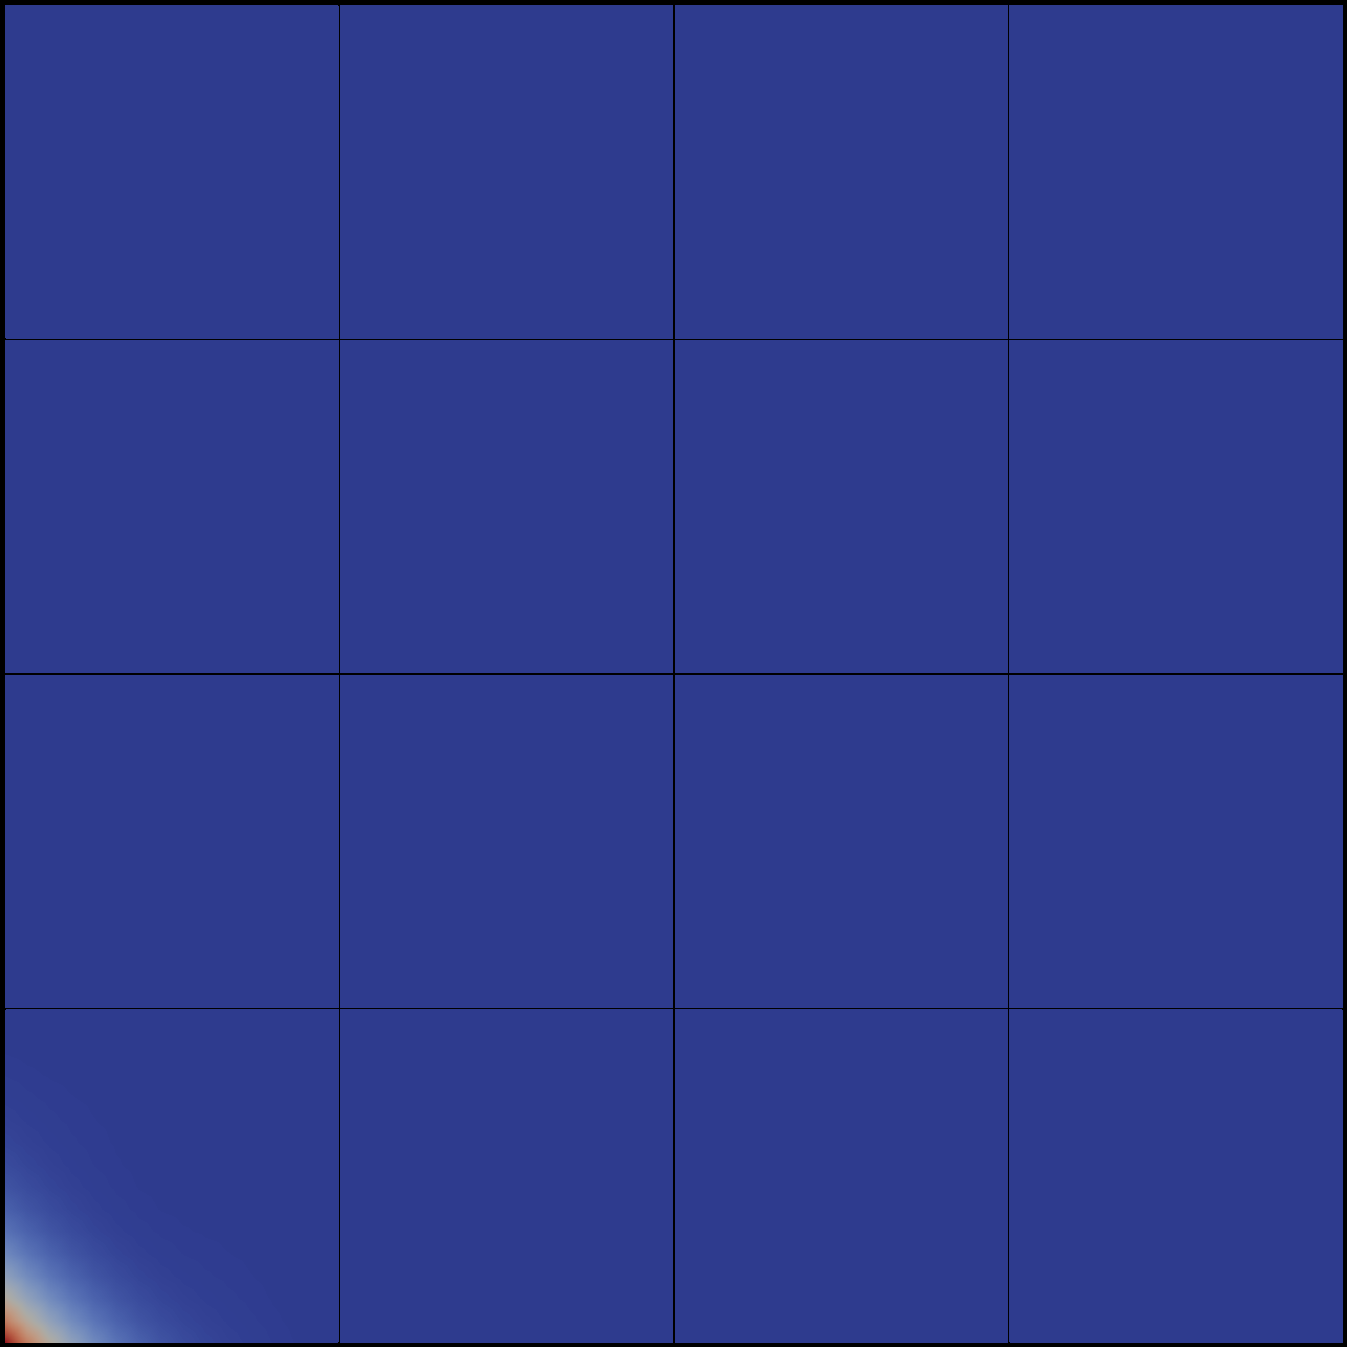
\includegraphics[width=0.45\textwidth]{Chapter_adaptive_mesh_refinement/media/load_imbalance_initial} \label{fig:mesh_imbalance_initial}}
	\hfill
	\subfloat[Mesh after refining]
	{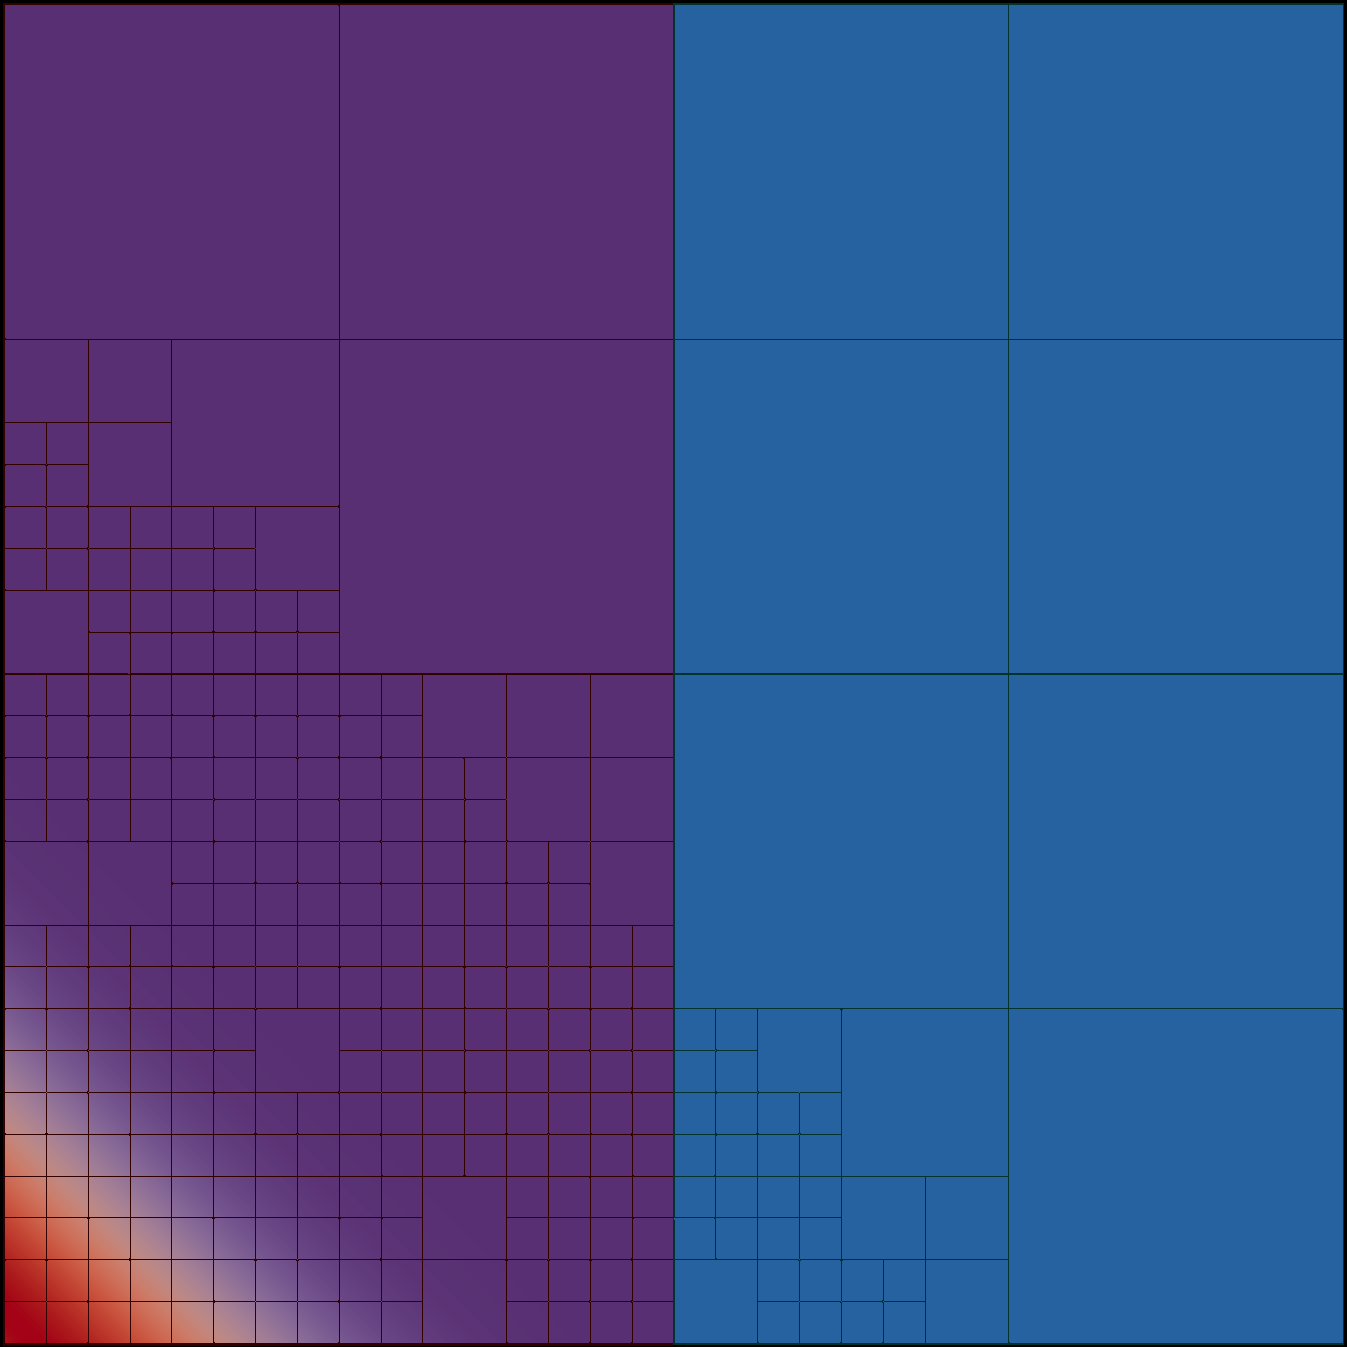
\includegraphics[width=0.45\textwidth]{Chapter_adaptive_mesh_refinement/media/load_imbalance} \label{fig:mesh_imbalance_after_refinement}}
	\caption{Load imbalance: The elements have split unequally in the two worker GPUs, one having a higher computational load. (a) Before refining (b) After refining}.
	\label{fig:load_imbalance}
\end{figure}

One last potential issue with AMR is the appearing of load imbalance. For example, the mesh from
Figure~\ref{fig:mesh_refinement} is split in two blocks for two GPUs to work in parallel, as shown
on Figure~\ref{fig:load_imbalance}. Initially, both the left and right GPUs have the same number of
elements in their domain. After refining, the left GPU has more elements as the wave is in its
domain and more elements have split there. Elements will have to be sent from the left GPU to the
right GPU in order to even out the computational load, while ensuring that there are as few
interfaces as possible between the GPUs. Interfaces need to be minimised because the GPUs need to
communicate every timestep when computing fluxes on these interfaces. This involves transfers from
from the GPUs to their CPU, between CPUs, and finally back from the CPUs to their GPU for both
directions. This is an expensive process, and improving locality of the elements will help reduce
the runtime of that part of the computation. This is dynamic load balancing, and
Chapter~\ref{chapter:load_balancing} is dedicated to solving this problem.

\section{Error Estimation} \label{section:adaptive_mesh_refinement:error_estimation}

We can't simply refine everywhere in the domain at every occasion, else this is no better than
having a finer mesh to start with. The mesh must only be refined

\cite{Mavriplis1990}

\section{Refinement Criteria} \label{section:adaptive_mesh_refinement:refinement_criteria}

\section{Mortar Element Method} \label{section:adaptive_mesh_refinement:mortar_element_method}

\cite{Maday1989}

\section{Implementation} \label{section:adaptive_mesh_refinement:implementation}

As detailed in Chapter~\ref{chapter:graphics_processing_units}, the grid is stored on the GPU as a
flat array of elements, each element having pointers to its solution arrays, stored in GPU dynamic
memory. This ensures the elements have a fixed size regardless of their polynomial order.